\section{Analysis and Interpretation} \label{sec:res-analysis}

This section analyzes and assesses the results of experiments conducted on GANmix. The evaluation identifies trends, investigates potential future directions for research, and interprets the results in the context of the research goals and the broader field.

\subsection{Identifying Trends}

Examination of the experimental results reveals several patterns and trends. There is an inverse correlation between generator and discriminator losses; as one increases, the other decreases. However, in certain cases both losses decrease together, which is beneficial. Also, convergence tends to plateau after a certain number of epochs.

This can be seen in Figure~\ref{fig:exp1_loss}. There, it can be seen that the loss of the generator decreases as the loss of the discriminator increases, and then the opposite occurs. Eventually both losses level off and decrease slightly.

The study found that the speed of convergence was affected by the learning rate. Although higher learning rates led to a faster convergence plateau, they did not necessarily lead to better results. This was demonstrated in Experiment 2 (Section~\ref{sec:exp2}), where the learning rates were increased and a loss plot is observed that is similar to Experiment 1 (\ref{sec:exp1}), but with a significantly faster plateau.

In Experiment 4 (Section~\ref{sec:exp4}), it appears that \ac{SGD} initially outperforms RMSprop, although it learns at a significantly slower rate. The results seem to be similar to Adam. Given the limited training time, one can only make assumptions, but it seems that using \ac{SGD} as the optimization algorithm leads to better performance than alternative methods such as RMSprop and Adam, despite the slower convergence.

Regularization methods such as dropout, batch normalization, and Gaussian noise have been shown to improve results and extend convergence, as shown in Experiment 5 (\ref{sec:exp5}). Although the spectrogram was suboptimal, the loss curves showed a healthy trend, with both losses decreasing consistently over time. Although the application of the elastic net regularization presented some challenges, it showed promise. The model performed better overall and achieved faster convergence when the generator and discriminator had similar parameter sets.

It was determined that larger models resulted in more rapid and resilient convergence. However, it should be noted that achieving satisfactory results was critically impacted by the size of the dataset. Typically, larger datasets and models produced better outcomes.

The embeddings generated by AudioLDM's \ac{VAE} show similarities characterized by a normal-like distribution with a significantly low standard deviation. Figure~\ref{fig:original-latents-hist} shows a histogram of these values, which extend to hundreds on the x-axis due to the residuals. It can be seen that the distribution is predominantly concentrated in an area close to zero.

\begin{figure}[ht]
    \centering
    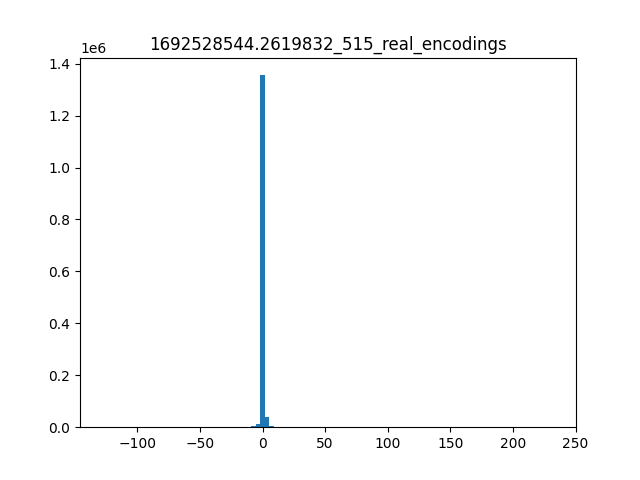
\includegraphics[width=0.6\textwidth]{figures/4.5-results/real_distribution.png}
    \caption{An histogram that represents the latent values created by AudioLDM's \ac{VAE}.}
    \label{fig:original-latents-hist}
\end{figure}

Experience 10 (\ref{sec:exp10}) showed an interesting trend. However, it is worth noting that although the generated spectrograms showed improvement, the generator loss increased while the discriminator loss consistently decreased after a few epochs, as can be seen in Figure~\ref{fig:exp10_loss}. The use of linear layers instead of convolutions proved to be advantageous in generating more robust spectrograms. Further investigation is needed to determine if there are problems with the optimizer.

This last experiment, which used linear layers, produced the most encouraging results and was chosen as the primary study for this dissertation.

\subsection{Results for Future Investigation}

In some experiments, a decline in performance after a few epochs was observed, resulting in losses becoming \ac{NaN}. This is seen in Experiments 8 and 9 (Sections~\ref{sec:exp8}, \ref{sec:exp9}). Further research is required to determine the underlying cause and prevent this occurrence in future experiments.

The impact of elastic network regularization on model performance requires further investigation. Despite the implementation challenges encountered, the initial results suggest that this regularization method has improved and shows potential effectiveness.

In addition, the issue of the continuously increasing generator loss in the last experiment requires further investigation in the future.

\subsection{Interpretation of Results}

The study's findings did not meet the expectations set forth in the thesis as the generated sounds are not state-of-the-art for generative models; however, they are encouraging. With sufficient data and time, the model has the potential to generate high-quality sound. This suggests that generative \ac{AI} models, especially \acp{GAN}, have significant capabilities in audio generation.

Furthermore, exploring the model's latent space is seen as a promising strategy for achieving better results. The latent space method is a simpler approach that can potentially yield more favorable outcomes for future models.

The limitations of the small datasets used in this analysis are evident. The bigger one, Clotho, comprised sounds lasting from 15 to 20 seconds, but with 5 seconds removed from each sound, certain sounds were too short to produce satisfactory results.  Additionally, the total sound count in the data set was less than 5,000, which isn't enough to properly train a generative model.

Thus, a significant concern uncovered in this study is the lack of an appropriate dataset. To achieve more precise results, it is critical to have access to comprehensive datasets. Nevertheless, it is imperative to recognize that the process of training models on large data sets involves significant computational resources that may not be readily available.

\subsection{Conclusion}

In summary, the analysis and interpretation of the data show trends and patterns observed in the experiments. The results did not meet initial expectations; however, they show potential for future advances in generative \ac{AI} models for audio synthesis. It is important to note that comparisons with state-of-the-art audio generation models are not discussed in this study due to the unsatisfactory practical results obtained. 